\chapter{A process overview}

\begin{center}
  \textit{If you can't describe what you are doing as a process, you don't 
          know what you're doing.}

 - W. Edwards Deming
\end{center}

This chapter will describe the NMR data analysis process in detail,
including the roles of computational and manual analysis, their interaction
with the data types, and tools used in the process.
In order to study proteins in solution using NMR, multi-step processes are 
employed to collect and analyze data.  An example process is shown in 
Figure \ref{nmr_overview} as a series of independent stages 
\cite{guerry2011automated}.
Figure \ref{process_timeline} shows a view of the process in the context
of the data discussed in the previous chapter.



\section{Data Collection}

See panel A of Figure \ref{nmr_overview}.

\subsection{Sample preparation}
The protein or molecule of interest is isolated and a solution 
obtained.  The preparation procedure employed will determine isotope labeling
and concentration.

\subsection{Time-domain data acquisition}
The solution is placed in an NMR spectrometer and an array of pulse sequences
are used to collect time-domain data.

The collection of data suitable for Fourier Transform processing, described
in the next section, requires uniformly collected data in each dimension.

Sensitivity, which determines the ability to discern true signals
from noise in the frequency domain, places constraints on data collection
\cite{rovnyak2004accelerated}.  Non-uniform sampling approaches 
\cite{maciejewski2011random} avoid these tradeoffs by collecting more data
points where the signal-to-noise ratio is high, but maintain resolution by
still collecting some data points where the signal-to-noise is low.


\section{Spectral processing}

In Figure \ref{nmr_overview} panel B, 
spectral processing operates on these FID data sets.  They are 
converted to frequency-domain spectra using tools such as NMRPipe \cite{nmrpipe}
and the Rowland NMR ToolKit \cite{rnmrtk}.  Functions such as 
zero-fills, Fourier transforms, phase shifts, apodizations, and linear 
predictions are applied to the data as a processing pipeline.  These 
functions are used to ensure that the spectra are amenable to further 
analysis, by optimizing peak size and shape and minimizing processing 
artifacts.

The raw data collected from an NMR spectrometer is referred to as 
time-domain data.  In a typical NMR experiment, these data represent the 
sum of multiple decaying sinusoids.  These FIDs are converted to 
frequency-domain spectra which are used in further analysis.  The goal of 
this phase is to construct a frequency spectrum which indicates the resonance 
frequencies of the atoms that were observed in the experiment.  A common tool 
for such a transformation is the Fourier Transform, which is able to convert 
a uniformly collected data set into a frequency spectrum.  
An example of an NMR spectrum of N-H groups is shown in Figure \ref{nhsqc}.
Due to relaxation decreasing the amplitude of an NMR signal over time, peaks 
have an intrinsic linewidth in the frequency spectrum.

Alternative approaches include multidimensional decompsition \cite{mdd}
and maximum entropy reconstruction \cite{hoch1996nmr}.  When FIDs are 
non-uniformly collected, these processing methods are required.

Considerations include minimization of processing artifacts, signal-to-noise 
ratio, accounting for water lines, avoiding rolling baselines and baseline 
offsets, linewidth and shape, phasing, and apodization.  Multiple software 
packages exist for carrying out this conversion \cite{nmrpipe, rnmrtk}.
These packages include functions for processing the data in specific ways to 
guarantee desirable qualities.  A typical procedure for spectral processing 
involves the sequential application of multiple functions from one of these 
packages.  At each stage, the input is a data set and associated metadata, 
which includes information such as spectral width, dwell time, and number of 
points.  Each function may require the setting of one or more parameters in 
order to proceed.  Thus, in addition to the final frequency-domain spectrum, 
the process generates several intermediate data sets, several 
intermediate metadata sets, and the sequence of functions used along with 
their parameterizations.  Previous work from our lab has enabled the 
convenient collection of necessary metadata during spectral 
processing \cite{connjur-wb}.



\section{Spectral analysis}

In the spectral analysis stage, Figure \ref{nmr_overview} panel C,
the overall goal is to identify the chemical shifts of individual atoms.
The spectra may be analyzed using a tool such as XEasy \cite{xeasy}, 
Sparky \cite{sparky}, NMRViewJ \cite{nmrviewj}, or CCPN Analysis \cite{ccpn}.  

In each spectrum, peak-picking is performed, and true signal peaks must 
be identified and separated from peaks caused by noise and artifacts.  
Additionally, signal peaks caused by contaminants must be identified.  
Next, GSSs are identified and constructed \cite{ccpn}. 
The connectivity of resonances in a GSS is exploited 
in through-bond experiments.  GSSs then must be assigned 
connectivities to other GSSs through overlap of mutual resonances, 
amino acid types, and finally specific residues of the sample of interest. 
Resonances must also be assigned to specific atoms \cite{ccpn}, 
with the final result being that specific atoms in the sample of interest 
are assigned chemical shift values.  Currently, 100\% assignments are not 
achievable due to several factors such as data quality, ambiguity,
missing resonances, and metal ions \cite{guerry2011automated}.
Between 80\% and 95\% completion may be required \cite{williamson2009automated}
for successful analysis at later stages.

\subsection{Peak picking}
Peak picking is the process of identifying and characterizing the peaks in 
a spectrum.  The goal is to identify all true signal peaks, while recognizing
and separating false peaks.

To a first approximation, a peak is identified by a local maximum in the 
frequency spectrum.  However, not all local maxima are necessarily true
peaks: noise and artifacts give rise to false peaks.  Nor do all peaks show 
up as local maxima if 
they are weak and close to the noise level, which causes them 
to be nearly indistinguishable from the noise and baseline; this may be due to 
sample instability such as aggregation or precipitation, or low sample 
concentration \cite{picky, munin, korzhnev2001munin, apart, autopsy, pine}
\cite{williamson2009automated, guntert2009automated, altieri2004automation,
baran2004automated}.
Each peak cross section has a non-zero width; adjacent signals may give rise
to overlapping peaks, distorting measurement of their attributes and possibly
also leading to disappearance of a local maximum.
Figure \ref{nhsqc_peaks} shows a portion of a peak-picked
NHSQC spectrum; note the overlap, and that some -- but not
all -- low-intensity spectral features have been identified as peaks.

Given these inherent issues, a general strategy for peak picking is 
described in \cite{autopsy, picky} and summarized here.
First, the noise level is estimated and points below the noise are discarded.
Next, of the remaining spectral regions, isolated areas are picked as peaks.
Finally, overlap is resolved by lineshape matching, the peaks are picked
and their attributes measured.  An optional additional step is filtering
based on symmetry and linewidth \cite{autopsy, picky}.

Correct peaks are important because they form the basis for the construction 
of GSSs, the assignment of chemical shifts to atoms, and the interpretation of 
NOESY spectra which give rise to distance restraints as a preliminary to 
structure calculation \cite{guerry2011automated}.  
Incorrect peak identification or position can result 
in misinterpretation of NOESY spectra, which could lead to false distance 
restraints between atoms which are in fact very far apart in the actual 
protein structure.

Estimates of the amount of false positive and false negative peaks picked 
by computational tools range from low (10-40\%) to high (70-135\%) \cite{pine}. 
The quality of the results generally depends on characteristics of the 
spectrum, especially the signal/noise ratio, and resolution, as well as 
characteristics of the molecule including \mattfttwo{} (which has an 
effect on peak width) and number of atoms -- more atoms give rise to
more peaks, and therefore a higher chance of overlap.

Since none of these approaches yields perfect 
results \cite{guerry2011automated}, manual intervention during peak picking 
is important for obtaining results of sufficiently high quality
\cite{guntert2009automated}; many peak picking 
programs allow and encourage semi-automated interaction in order to clear 
up troublesome spectral features.  
Manual intervention is often accomplished based on knowledge outside of the 
spectrum: existence, position, and shape of peaks in other spectra, knowledge 
of the solvent, characteristic artifactual patterns caused by a specific 
processing scheme, knowledge of the local dynamics of a small region of the 
protein.  \cite{williamson2009automated, guntert2009automated, 
altieri2004automation, baran2004automated}
Because of this, peak picking can often not be completely finished until 
later analysis has been accomplished.

\subsection{GSS and resonance construction}
As many pulse sequences are specificially designed to exploit the strong
backbone H-N coupling and correlate additional nearby atoms, H-N groups appear 
in many through-bond spectra and are given a privileged position in analysis: 
the signals which H-N groups give rise to appear at matching chemical shifts
across multiple spectra.
This H-N matching enables grouping of peaks into GSSs; given multiple spectra
which include N-H dimensions, peaks with matching N and H chemical shifts are
determined to belong to the same GSS.
Table-\ref{pulse_sequences} shows that H-N chemical shifts are captured in 
multiple spectra, and sometimes multiple times within a single spectrum.
At a later stage, GSSs are often augmented with additional sidechain resonances.
	
In addition to GSSs of backbone resonances, H-N-rooted GSSs typically are 
visible for Asparagine and Glutamine sidechains, and smaller GSSs of 
Tryptophan sidechains are visible.  Arginine sidechains may also give rise 
to an H-N-rooted GSS under certain experimental conditions. 

The difficulty in constructing these GSSs correctly and unambiguously stems 
from the issues inherent in NMR data.  First, the success of the standard 
suite of experiments rooted in H-N -- NHSQC, HNCO, HNCACB, etc. -- depends 
on \cite{autoassign1997}: % page 600 -- `reliability`
\begin{enumerate}
  \item good dispersion, i.e. no overlap, otherwise it is difficult to determine 
    which peaks belong with which H-N-rooted spin system.
  \item the H-N chemical shifts being nearly identical across all spectra.  
    This may not be the case if there are variations in the sample or the 
    temperature.  The Bloch-Siegert shift and experimental error also can have 
    an effect on chemical shift.
  \item nuclei appearing at a single chemical shift.  If there are multiple 
    conformations or chemical heterogeneity \cite{autoassign1997}, 
    a nucleus may appear at multiple chemical shifts and appear to be two 
    different resonances.
  \item the presence of an H-N group -- Proline is a notable exception, and 
    so it does not show up in experiments which rely on the presence of an H-N group
  \item extraneous peaks which do not seem to fit into a spin system, or 
    peaks which do not seem to match peaks in other spectra
  \item accurate (or at least consistent) spectral referencing.  
    Misreferenced spectra will cause the same nucleus to show up at different 
    chemical shifts across multiple spectra.
  \item quality of peak-picking \cite{autoassign1997, mars}: 
    chemical shifts, lineshapes, as well as the numbers of 
    false positives, false negatives, extraneous peaks
\end{enumerate}

Computational approaches for GSS construction tend to require manual 
assistance in some cases \cite{autoassign1997, mars}.  Incorrect or 
incomplete GSSs will have negative effects on the quality of later 
analysis; several assignment tools assume that manual intervention will 
verify and, if necessary, correct the GSSs \cite{williamson2009automated}; 
this allows the tools to be conservative in their 
predictions \cite{autoassign1997}.  However, it may not be 
possible to unambiguously and completely construct GSSs until the results 
of later analysis are available: some approaches use NOESY peaks and 
assignments as well as structure results to verify and correct GSSs 
\cite{autoassign1997}.

Figure \ref{nhsqc_hncacb} shows an example of matching peaks between two
spectra.  The quality of the match -- how closely the chemical shifts line up,
as well as the lack of overlapping peaks -- means the peaks are easily
identified as members of the same GSS.

\subsection{Resonance typing}
Before assigning a resonance to a specific 
atom, the atomtype of a resonance may be assigned.  In an HNCO experiment, 
this is typically straightforward, because for each backbone spin system, 
the H dimension always corresponds to the backbone H, the N dimension always 
corresponds to the backbone N, and the C dimension always corresponds to the 
backbone C(i-1).  However, the situation is more complicated in an HNCACB 
experiment, as there are generally four choices of atomtype assignment for 
the C dimension:  CA, CB, CA(i-1), and CB(i-1).  Thus, the resonance given 
by the C dimension of each peak must be assigned one of these choices.  
Reasons for choosing a specific assignment include peak sign, as well as 
chemical shift compared to statistics available in the BMRB.  In addition, 
the overlap between experiment pairs such as the HNCACB and CBCA(CO)NH 
facilitates resonance-atomtype assignment: while the CA(i-1) and CB(i-1) 
are expected to appear in both experiments at the same chemical shift for 
a given backbone H-N root, the CA and CB are expected to appear only in the 
HNCACB spectrum.

\subsection{GSS typing}
Correspondingly, GSSs are also assigned amino acid types.  This phase 
interacts strongly with the assignment of atomtypes to resonances, in 
that the possible atomtypes to which a resonance may be assigned depends 
on the amino acid type, and the expected chemical shift ranges for various 
atomtypes depends on amino acid type as well.  For instance, GSSs assigned 
to the Glycine amino acid type should not have a CB; and the CB resonance's 
chemical shift of a GSS assigned to Alanine is expected to be very different 
from all other CB chemical shifts.  Backbone amino acid types may be split 
into several categories \cite{saga} based on BMRB statistics for 
CA and CB chemical shifts \cite{bmrb}:
\begin{enumerate}
  \item Ala
  \item Gly 
  \item Pro
  \item Ser, Thr
  \item Val, Met, Lys, His, Arg, Glu, Gln, Trp, Cys
  \item Asp, Asn, Ile, Leu, Phe, Tyr
\end{enumerate}
However, GSS typings are complicated by several factors.  First, GSS typing 
requires correct and complete GSS construction.  Second, correctly assembled 
GSSs may include overlapped or extraneous peaks, expected peaks (based on a 
spectrum's typical results) may also be missing.  Third, most GSSs can not 
be uniquely typed based solely on CA and CB chemical shifts, as groups 5 and 
6 (above) as well as 4 are ambiguous.  Fourth, sidechain GSSs must be 
identified and separated.

\subsection{Sequential GSS assignment}
Sequential GSS assignments exploit the previously mentioned overlap of pulse
sequences such as the HNCACB and HN(CA)CO.  Sequential GSSs 
are expected to have CA/CA(i-1), CB/CB(i-1), and CO/CO(i-1) resonances at 
identical chemical shifts.  This duplication enables sequential assignment 
of GSSs.  Note that there is substantial interaction between atomtype-resonance 
assignment and sequential GSS assignment: assigning two GSSs sequentially 
implies the CB vs CB(i-1), CA vs CA(i-1), and C vs C(i-1) atomtype assignments 
of the resonances in both GSSs; knowing the atomtype-resonance assignments of 
two spin systems can prevent their sequential assignment (if, for example, the 
matching resonances are both CB(i-1)); and not knowing the atomtype-resonance 
assignment implies that the sequential GSS assignment may be invalid.  
Sequential GSS assignment is complicated by: 
\begin{enumerate}
  \item missing peaks, possibly caused 
  by local dynamics, which reduce the number of overlapping resonances between 
  potential sequential GSSs, and can also disrupt atomtype assignments of 
  resonances; 
  \item extraneous peaks, which may be false positives or caused by 
  multiple conformations of the protein, causing incorrect matches
  \item degeneracy of chemical shifts:  given two GSSs with identical CA(i-1) 
  and CB(i-1) resonances, as well as a third GSS with matching CA and CB 
  resonances, it is impossible to unambiguously assign sequentially solely 
  on the basis of chemical shift matching between the two GSSs 
  \cite{autoassign1997}.
\end{enumerate}

An example of GSS overlap is shown in Figure \ref{hncacb_overlap}.  Green peaks
are CA, and purple peaks are CB; note that one each of green and purple peaks
match between the two GSSs.

\subsection{Sequence-specific GSS assignment}
Since backbone GSSs are H-N-rooted, a GSS is assigned to a 
backbone-amide; this implies the assignment of resonances to atoms as well, 
based on matching of atomtypes.  When a typical GSS is assigned to a residue, 
the H, N, C, C(i-1), CA, CA(i-1), CB, and CB(i-1) atoms will be assigned 
resonances as well.  Sequence-specific assignment interacts heavily with 
sequential GSS assignment, because the protein sequence must be compatible 
with the GSS sequence, where `compatible' means that the amino acid types 
of the GSS match those of the protein sequence.  Note that full assignment 
of amino acid type to GSS is not a prerequisite for GSS-residue assignment; 
in fact, GSS-residue assignment may lead to GSS-amino acid type assignment 
for sequentially connected GSSs.  GSS-residue assignment is facilitated by 
long chains of sequential GSSs in which some of the GSSs are typed as Serine, 
Threonine, Glycine, or Alanine.  The longer a GSS chain, the fewer places it 
might possibly fit into the protein sequence \cite{saga}.  Also, 
as sequence-specific assignment proceeds, the number of unassigned GSSs and 
residues decreases; the result is that initially ambiguous assignments become 
unambiguous as choices are removed.  Conversely, complications arise from 
incomplete sequential GSS assignments resulting in short, ambiguous chains.  
The presence of prolines generally ends chains due to the lack of a backbone 
H-N group.  Missing GSSs also terminate chains.  Relatively few Ser, Thr, Gly, 
and Ala residues means the number of unambiguous anchor points will be lower.

Figure \ref{ss-residue} shows an example of sequence-specific GSS assignment.
Although not all of the GSSs have been typed, the presence of a Glycine and
Serine in the GSS chain reduces the possible assignments to residues.
Additionally, the length of the GSS chain helps reduce the ambiguity compared
to shorter GSS chains.

\subsection{Sidechain: spin system and resonance assignment}
The next group of experiments collects chemical shifts of sidechain atoms.  
These experiments include 
the HBHA(CO)NH \cite{hbhaconh} in Figure \ref{ccpn_hbhaconh}, 
the C(CO)NH-Tocsy \cite{cconhtocsy} in Figure \ref{ccpn_cconhtocsy}, 
the HC(CO)NH-Tocsy \cite{hcconhtocsy} in Figure \ref{ccpn_hcconhtocsy}, 
the HCCH-Tocsy \cite{hcchtocsy} in Figure \ref{ccpn_hcchtocsy}, 
and aromatic Tocsys.  The purpose of these experiments is to 
obtain the chemical shift values of sidechain resonances of protons, since 
proton frequencies are necessary in order to interpret NOESY spectra.  To 
interpret these spectra, the peaks must be assigned to GSSs and atomtypes 
must be assigned to the new resonances. While several of these experiments 
are also rooted in backbone H-N groups, facilitating the addition of peaks 
to the correct GSS, others -- such as the HCCH-Tocsy -- are not.  These are 
analyzed by the matching of resonance chemical shifts with those from other 
experiments targeting sidechains.  Atomtype-resonance assignments can generally 
be made with reference to compiled BMRB statistics.  Complications in this 
phase include: stereospecificity -- nuclei such as HA2 and HA3 may give rise 
to different chemical shifts, but resolving the correspondence may be 
impossible without further data; overlap -- especially in the HCCH-Tocsy 
where sidechains of the same amino acid type but different residue may have 
many closing matching chemical shifts; overlap between resonances within the 
same GSS, especially in Leu and Ile; missing and extraneous data; and the 
difficulty of both obtaining and unambiguously interpreting aromatic data.  
New approaches for sidechain data collection and assignment have recently 
been developed \cite{mobli2010non, hiller2008apsy} which seek to address 
these issues by reducing ambiguity of chemical shifts.

\subsection{Alternative approach: probabilistic assignment}
The previously described approach views analysis as a pipeline: input is 
transformed into output, which becomes the input for the next stage, and so on.  
PINE \cite{pine} removes the pipeline constraint by connecting each stage to 
each other and allowing information to flow freely; this enables statistical 
weighting of interpretation as well as dependencies such as peak picking 
on GSS construction (a dependency which is not possible in the pipeline 
approach).  PINE does not remove the need for manual intervention; it is
still assumed that some level of intervention is necessary to obtain the
best results \cite{pine}.


\section{Structure determination}

In the final stage, Figure \ref{nmr_overview} panel D, the chemical shift 
assignments are used to interpret the NOESY experiments and a structure
is calculated and refined.

\subsection{NOESY peak-picking and assignment}
NOESY peaks provide structural restraints if it can be 
determined which protons gave rise to the peak.  Analysis of NOESY spectra 
therefore requires chemical shift assignments of atoms to 
determine the protons involved in a peak.  
NOESY spectra are  processed and peak-picked, similarly to through-bond 
spectra, and resonance assignments of peaks made.  
Considerations used to analyze 
NOESY spectra include: symmetry -- a peak is expected to correspond to a 
matching peak with the frequencies of the two 1H dimensions swapped; patterns 
based on known proximity of atoms from the primary sequence giving rise to 
many short-distance NOE peaks; network anchoring.  Complications include 
overlap caused by degenerate chemical shifts of protons, leading to 
ambiguous interpretations of peak assignments; this can be greatly mitigated 
by the use of an extra dimension:  15N- or 13C-edited NOESY spectra reduce 
the ambiguity, as well as incorrect or incomplete chemical shift assignments.

NOESY assignment may be done automatically \cite{cyana2004, aria2003}.  
NOESY peak-picking may be automated as well \cite{munin, korzhnev2001munin}.

An alternative approach is taken by ABACUS \cite{abacus_assignment}, which uses
Monte Carlo probabilistic methods for assignment, NOE assignment, and structure
calculation.  However, it is important to note that ABACUS still requires 
correct NOE peak picking and GSS construction as a prerequisite.

\subsection{Structure calculation}
The resonance assignments of the NOESY data are 
interpreted to obtain distance restraints, which are then used to calculate 
coarse-grained three-dimensional structures.  The structures may then be 
refined and fine-tuned using a computational tool such as Amber \cite{amber}.  
Unambiguous resonance assignment of NOESY data purely on the basis of chemical 
shift assignments may often be impossible or impractical, due to degenerate 
chemical shifts and to non-stereospecific assignments.  While these 
ambiguities can often be resolved through the collection of additional 
NMR data, the expense involved in doing so may often make it more practical 
to attempt to resolve the ambiguities through a structure determination 
program such as CYANA \cite{cyana2004}.

Cyana is able to calculate a three-dimensional structure from NOESY peaks, 
chemical shift assignments, and distance restraints \cite{cyana2004, aria2003} 
using an iterative approach to NOESY peak assignment and building structural 
models.  It also requires secondary structure information as input; as
chemical shift values are correlated to secondary structure, as described
by secondary chemical shift statistics \cite{spera1991empirical}, secondary 
structure can be calculated from chemical shift assignments using a program 
such as Talos \cite{talos+}.  Chemical shift assignments may also be used to 
calculate potential structures \cite{cs-rosetta}.  Additional programs 
may be used to refine structures \cite{amber, xplor-nih}.



\section{Discussion}

The inherent NMR issues of ambiguous, missing, and extraneous data cause 
problems throughout the entire analysis process.  Correctly dealing with 
these issues is difficult, but absolutely critical in order to obtain 
high-quality results \cite{williamson2009automated, guntert2009automated, 
altieri2004automation, baran2004automated}.  As yet, computational tools 
are not able to deal perfectly with these issues, due to one or more of 
several basic limitations: 
\begin{enumerate}
  \item they require high-quality input in order to function correctly 
  \cite{saga, abacus_assignment, mars, autoassign2001, ezassign, pine, cyana2004}; 
  this input is generally assumed to have been manually prepared in order 
  to meet the stringent quality requirements of completeness and absence of 
  extraneous results
  \item even with high-quality input data, tools are not able to produce 
  perfect results 
  \item tools perform differently in different contexts, although 
  performance generally decreases as protein size increases and spectral quality 
  decreases
  \item manual verification and correction of the results is assumed, 
  even for tools that claim to be fully automated 
  \cite{williamson2009automated, guntert2009automated, altieri2004automation,
  baran2004automated}
\end{enumerate}

A key limitation of many analysis tools is the fixed input data.  While
this simplifies the use of the tool in a simple pipeline, it may also lead
to reduced quality of results and explain the necessity of manual intervention:  
while the input data that a tool handles is restricted, manual interventions can
make use of any additional information required to make specific deductions. 
Thus, PINE and related efforts  
are an exciting effort to loosen these incidental restrictions.  Initial 
results are promising, and show a marked improvement, although manual 
intervention is still assumed to be necessary in order to obtain the best 
results \cite{pine}.  Further tools such as \cite{shiftx2, cheshire}, 
which calculate chemical shifts from structure,  
bring additional information to bear, helping to validate assignments.
Table \ref{data_connections} and Figure \ref{process_timeline} show some
of the key connections between various data types, putting these tools in
the overall context of NMR data analysis.

Another exciting development is the rise of probabilistic methods 
\cite{saga, pine}.  These methods reflect the reality that the 
confidence of a specific interpretation depends on the exact state of the 
data; in other words, an assignment which is 50\% confident given only an 
HNCA spectrum may become 90\% confident if an HN(CO)CA spectrum is added.  
The significance of this confidence level is that it enables easy tracking 
of ambiguous and/or low-confidence interpretations -- i.e. those that stand 
to benefit from collecting additional data sets.  By including confidence 
values on all assignments, an understanding of the troublesome areas is 
facilitated.  This helps to reduce the cost of cascading errors -- if the 
uncertainty is tracked as a confidence level, further interpretations based 
on a highly uncertain datum will also receive low confidence levels.  In 
addition, confidence levels are an alternative to the inherent balance 
between completeness and correctness -- it is no longer necessary to 
sacrifice one for the other \cite{autoassign2001, pine}.


\section{Conclusions}

The massive amount of data involved in a structure determination process --
often on the order of gigabytes -- necessitates the use of computational
tools for data management as well as efficiency of analysis.  To address
specific problems in the NMR analysis process, many software implementations 
of useful data processing algorithms have been created, distributed, and 
maintained in recent years 
(\url{http://nmrbox.org/NMRbox.org/Registry.html}, 
\url{http://nmrwiki.org/wiki/index.php?title=Category:Software}, 
\url{http://bmrb.wisc.edu/tools/prog\_corner.shtml}).  
Additionally, several groups have 
accelerated the process by producing software tools spanning and integrating 
multiple steps to decrease the necessity for time-consuming human intervention
\cite{abacus_assignment}.
This allows automated or semi-automated structure determination for small 
proteins.  Other groups have built integrated pipelines, using one specific 
tool for each step \cite{baran2004automated, sail_flya}, 
and allowing manual intervention at traditionally 
difficult stages.  Many recent methods re-envision structure determination 
as an iterative process, where the results of a later stage may require the 
researcher to re-evaluate or re-perform an earlier stage \cite{cyana2004}; 
this has been applied to interpretation of NOE-derived 
restraints \cite{aria2003}.  Altogether, the structure determination 
process can often take several months \cite{guerry2011automated}.

In general, while computational tools are able to deliver results relatively 
quickly compared to manual analysis, they may not be able to produce more 
accurate results, especially when the input data is low-quality, irregular, or 
otherwise problematic; this can result in false positives and negatives
\cite{williamson2009automated}.  This is a problem at every stage of spectral
analysis.

This has the consequence that NMR structure determination data analysis 
processes cannot be fully automated if high-quality results are required.  
An effective solution to this problem combines the strengths of the automated 
and manual approaches, in a semi-automated fashion:  computational tools are 
used to quickly perform the majority of analyses such as peak-picking and 
GSS construction, and manual analysis is used to clear up the 
relatively small number of cases involving ambiguities and errors caused 
by problematic or unclear data.  Thus, some amount of manual analysis may 
be required at all stages of the data analysis process 
\cite{guntert2009automated, williamson2009automated}.   
See Figure \ref{data_key} for an overview of the broad categories of data 
involved.

Manual analysis therefore plays a critical role in NMR data analysis, due 
to the inherent issues of analysis which complicate automated tools, and 
to the ability to bring sufficient context to bear to solve difficult cases.  
Manual intervention is assumed to be necessary by 
most tools, even automated ones, to ensure the completeness and correctness 
of results.  However, despite the importance that manual intervention plays 
in analysis, the specific modifications made and their reasons for -- 
which may be quite complicated -- are not captured \cite{guntert2009automated}.  
Thus, the metadata of manual intervention is lost, and analysis is 
irreproducible.


% tables
\clearpage
\section{Tables}

% TODO more examples
% TODO some inputs, outputs have multiple data types
\begin{table}[h]
    \begin{tabular}{ | c || c | c | c | c | c |}
    \hline
      Data                                      &  Example              &  Reverse example      \\  \hline
      FID -> spectrum                           &  Frequency-domain     &  NMRPipe, RNMRTK      \\  \hline
      Spectrum -> peaks                         &  Sparky peak picker   &  ???                  \\  \hline
      Peaks -> GSSs                             &  ???                  &  ???                  \\  \hline
      Sequence -> chemical shifts               &  ???                  &  ShiftY               \\  \hline
      Chemical shifts -> secondary structure    &  Talos                &  ???                  \\  \hline
      Chemical shifts -> tertiary structure     &  CS-Rosetta, Cheshire &  Sparta+, ShiftX      \\  \hline
      Chemical shifts -> NOESY assignments      &  Cyana                &  ???                  \\  \hline
      NOESY assignments -> structure            &  Cyana                &  ???                  \\  \hline
    \hline 
    \end{tabular}
    \caption{Connections between various data types.}
    \label{data_connections}
\end{table}



% figures
\clearpage
\section{Figures}

\begin{figure}[h]
  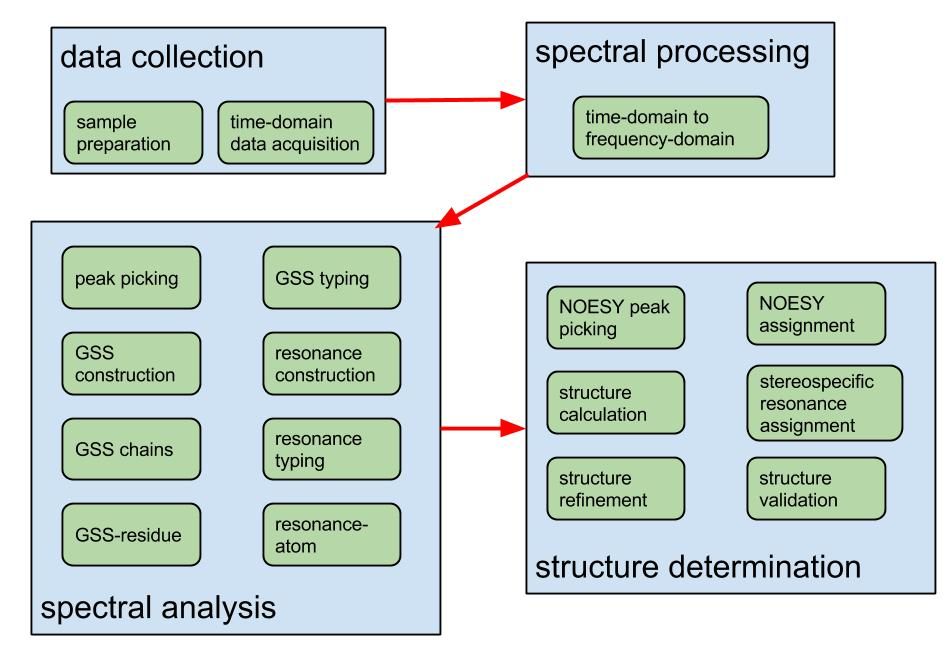
\includegraphics[scale=0.42]{figures/nmr_overview}
  \caption{An overview of the NMR process for protein structure determination}
  \label{nmr_overview}
\end{figure}

\begin{figure}
  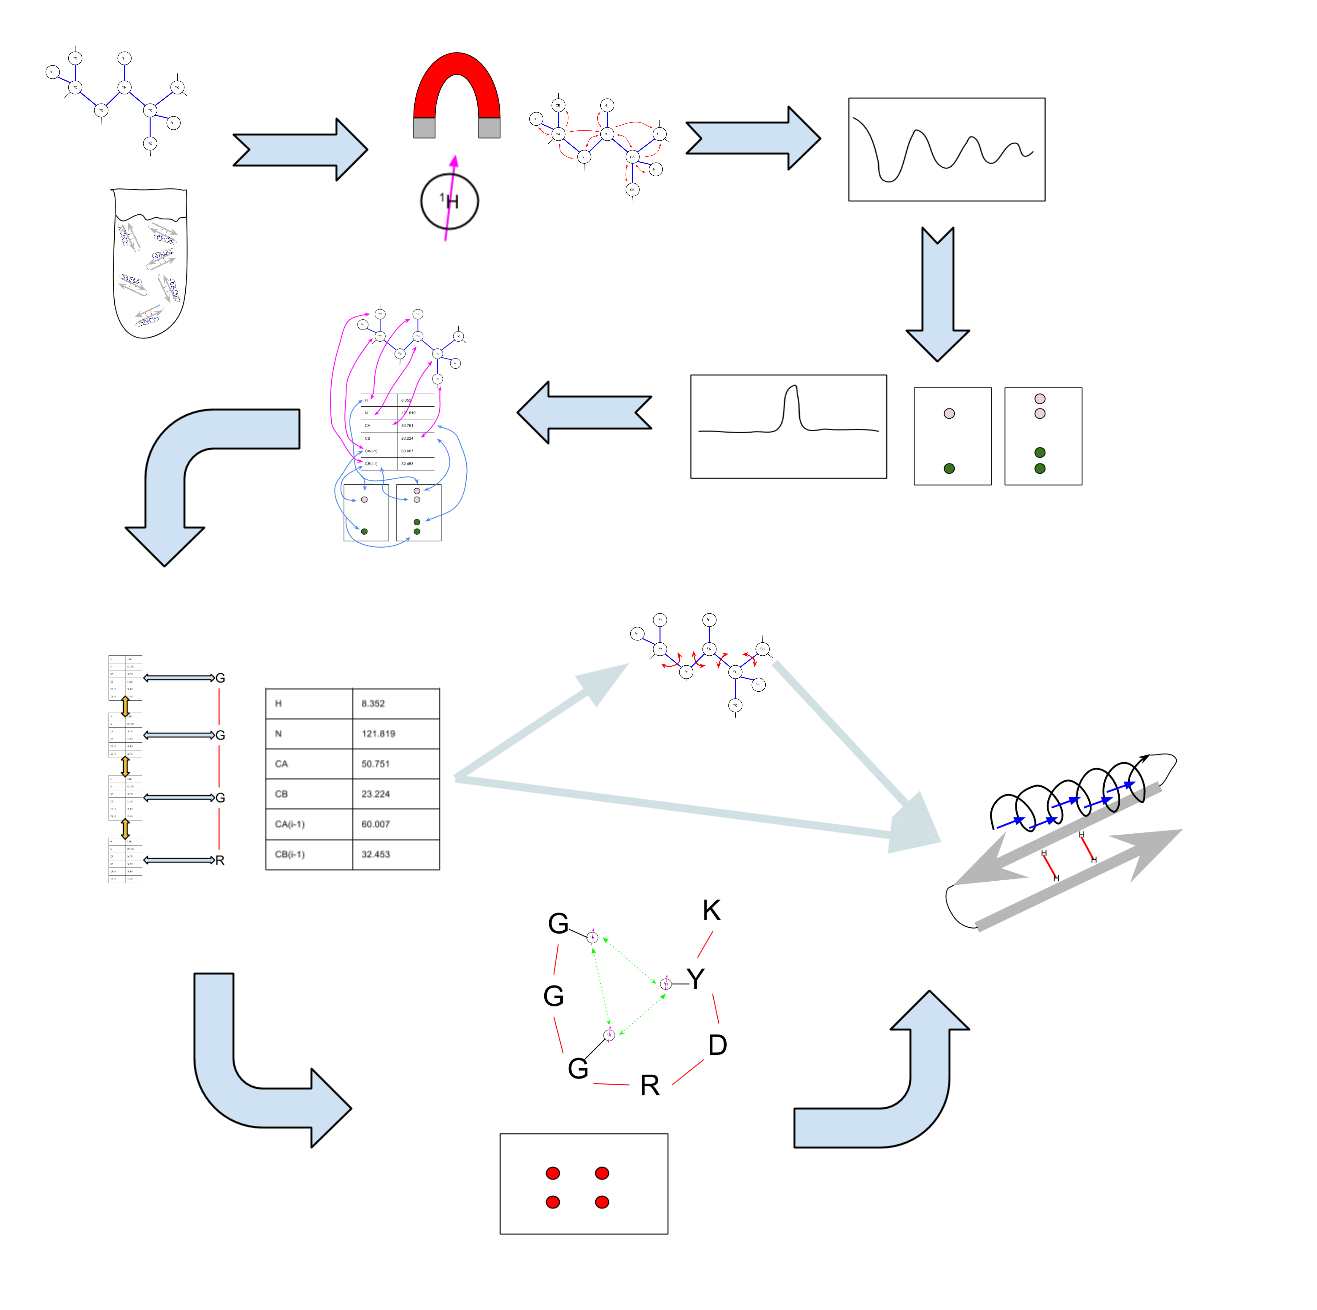
\includegraphics[scale=0.35]{figures/process_timeline}
  \caption{The connections between various data types.}
  \label{process_timeline}
\end{figure}

\begin{figure}
  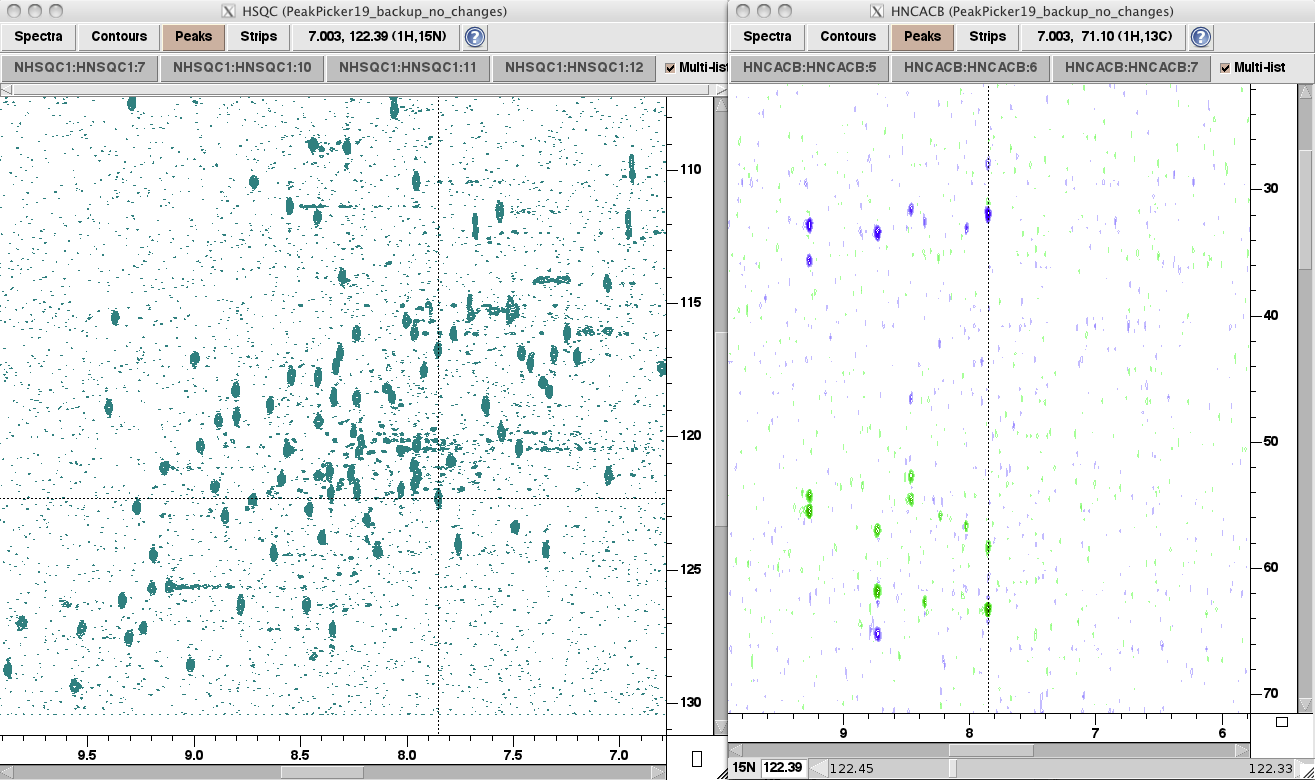
\includegraphics[scale=0.3]{figures/nhsqc_hncacb}
  \caption[Matching peaks between an NHSQC and an HNCACB spectrum]
          {Matching peaks between an NHSQC and an HNCACB spectrum.
           This likely indicates that the peaks belong to the same GSS.}
  \label{nhsqc_hncacb}
\end{figure}

\begin{figure}
  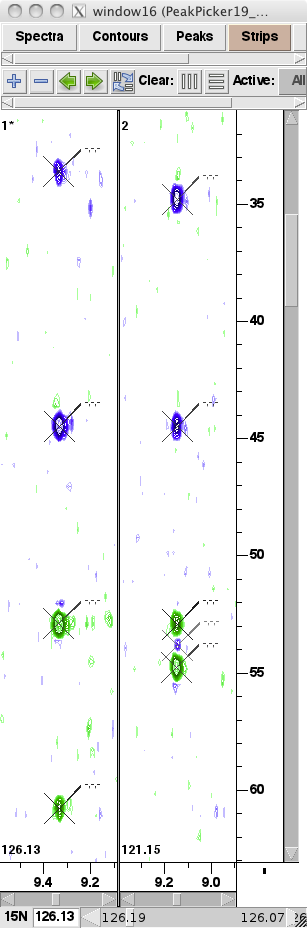
\includegraphics[scale=0.35]{figures/hncacb_overlap}
  \caption{Overlap of Carbon resonances in an HNCACB spectrum.}
  \label{hncacb_overlap}
\end{figure}

\begin{figure}
  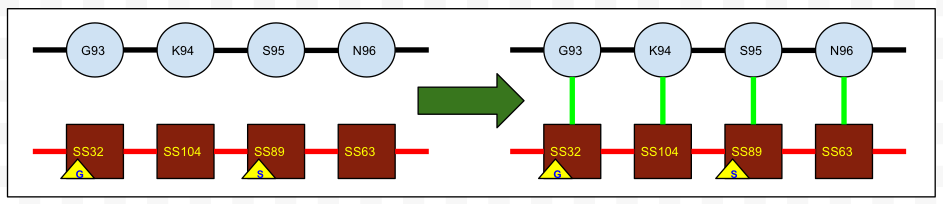
\includegraphics[scale=0.45]{figures/ss-residue}
  \caption[Assignment of a GSS chain to residues]
          {Assignment of a GSS chain to residues.  The circles are residues,
           black lines are peptide bonds, squares are GSSs, red lines are 
           sequential GSS assignments, and green lines are GSS-residue 
           assignments.}
  \label{ss-residue}
\end{figure}

\begin{figure}
  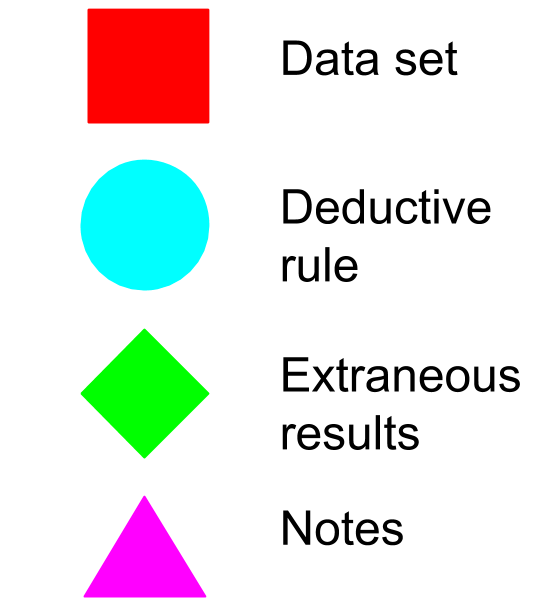
\includegraphics[scale=0.6]{figures/data_key}
  \caption{Categories of data used in the analysis process}
  \label{data_key}
\end{figure}

